\documentclass[11pt]{article}
\usepackage{report}

\begin{document}
\section{Introduction}
In this lab we will explore five different numerical methods for solving the wave equation
\begin{equation}
	\frac{\delta^2 u}{\delta t^2} = c^2 \frac{\delta^2 u}{\delta x^2}
\end{equation}
with three different initial conditions
\begin{equation}
	f(x) = exp(-(x-\frac{L}{2})^2)
	\label{eq:normal}
\end{equation}
\begin{equation}
	f(x) = sin( 2 \pi \frac{x}{L})
	\label{eq:sine}
\end{equation}
\begin{equation}
	 f(x) =\begin{cases}1 & \frac{10}{3}<x<\frac{20}{3} \\0 & else\end{cases} 
	\label{eq:square}
\end{equation}

One other part that is important is the so called CLF condition that will be referred to in the discussions
\begin{equation}
	\Delta t  \leq \frac{\Delta x}{c}
	\label{eq:clf}
\end{equation}
\section{Simple Explicit Method}

\begin{figure}[H]
	\centering
	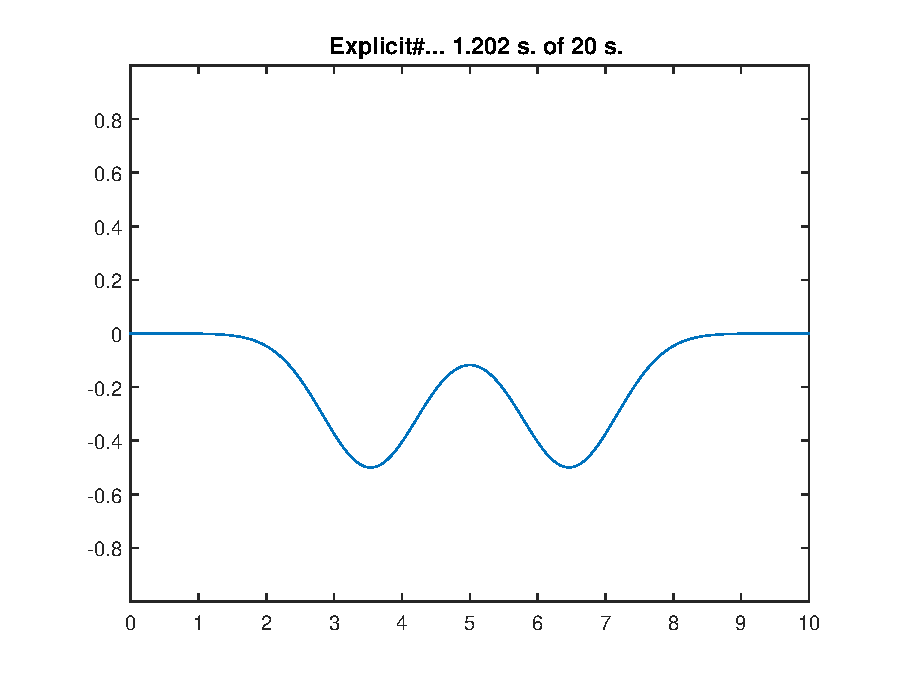
\includegraphics[width=1\textwidth]{../explicitNormal}
	\caption{Looking the explicit solving the wave equation with initial equation 
	\ref{eq:normal} 1.2 seconds into the simulation}
	\label{fig:explicitNormal}
\end{figure}
\begin{figure}[H]
	\centering
	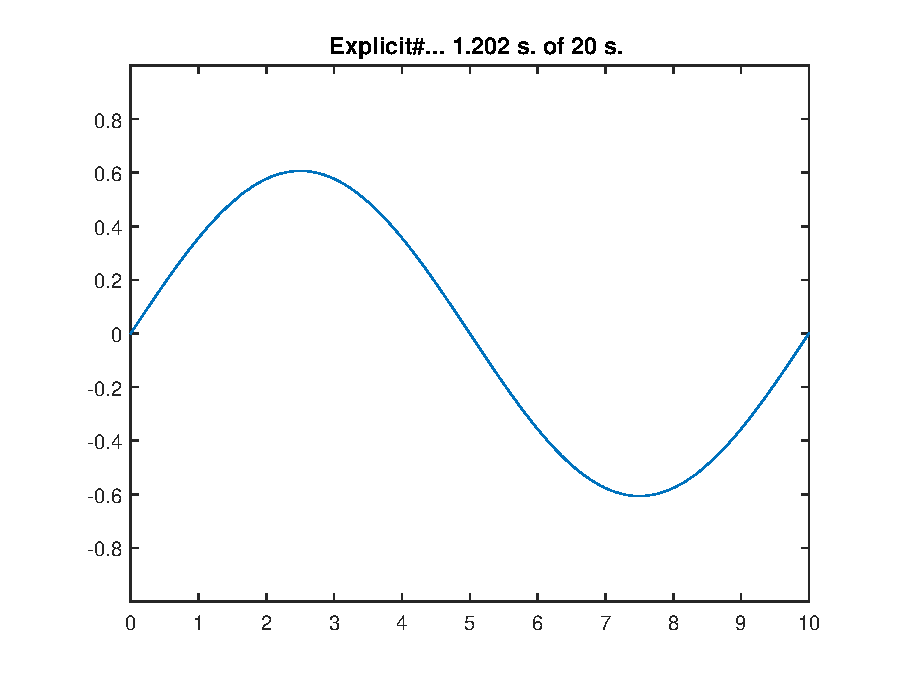
\includegraphics[width=1\textwidth]{../explicitSine}
	\caption{Looking the explicit solving the wave equation with initial equation 
	\ref{eq:sine} 1.2 seconds into the simulation}
	\label{fig:explicitSine}
\end{figure}
\begin{figure}[H]
	\centering
	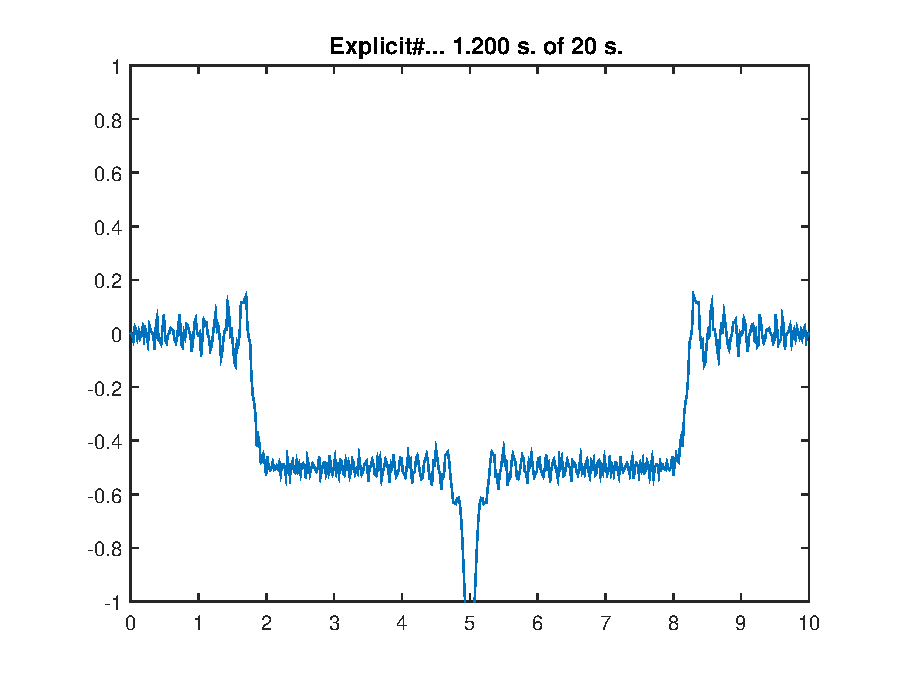
\includegraphics[width=1\textwidth]{../explicitSquare}
	\caption{Looking the explicit solving the wave equation with initial equation 
	\ref{eq:square} 1.2 seconds into the simulation}
	\label{fig:explicitSquare}
\end{figure}
Looking at the time step for this solver we can conclude that for the case with the initial condition of the equation \ref{eq:normal} and \ref{eq:sine} we can see very smooth results aslong as $\Delta t$ is no more then around 40\% bigger then the CLF condition (equation \ref{eq:clf}). It does not seem to matter if its lower then this. We seem to have no error amplification aslong as this condition is met. Not even damping is seen over 20 seconds using a time step that is half of what the CLF condition require.   

For the third initial condition, equation \ref{eq:square}, we could also go above the CLF condition with about 40\% without having the solution completly explode on us. But the solver had problem with the corners of the geometry. It caused some oscillations that was exaggerated if the time step was above the CLF condition. One should note though that the oscillation was always there, no matter if you where below the CLF condition. Below the CLF condition the size of the oscillation seemed to not change at all though, no matter how low time step one use.

All in all this shows that the simple explicit method is usable for solving the wave equation with a nice and smooth initial condition.  

\section{A Simple Fully Implicit Method}
\begin{figure}[H]
	\centering
	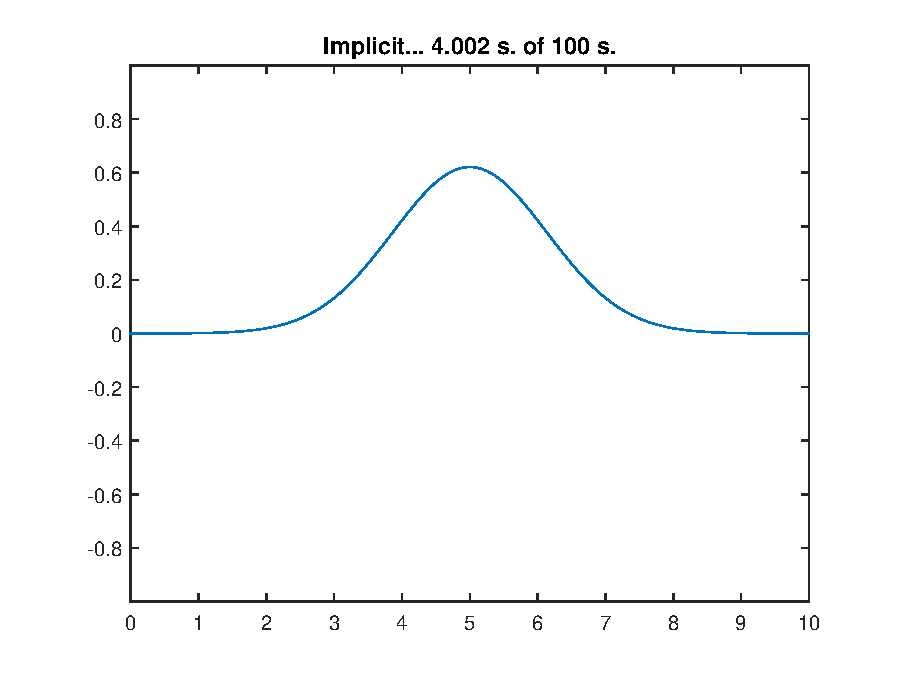
\includegraphics[width=1\textwidth]{../implicitNormal}
	\caption{Looking the implicit method solving the wave equation with initial equation 
	\ref{eq:normal} after a few periods. Note that in the initial period the "hill" touched the frame of the plot window, thus we have significant dampening}
	\label{fig:implicitNormal}
\end{figure}
\begin{figure}[H]
	\centering
	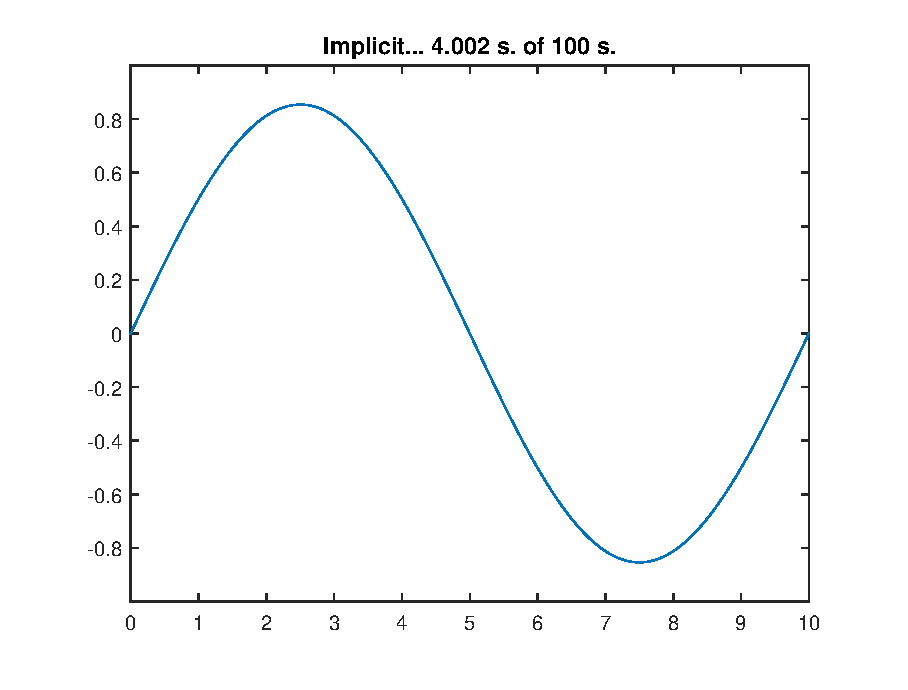
\includegraphics[width=1\textwidth]{../implicitSine}
	\caption{Looking the implicit method solving the wave equation with initial equation 
	\ref{eq:sine} after a few periods. Note that in the initial period the "hill" touched the frame of the plot window, thus we have significant dampening}
	\label{fig:implicitSine}
\end{figure}
\begin{figure}[H]
	\centering
	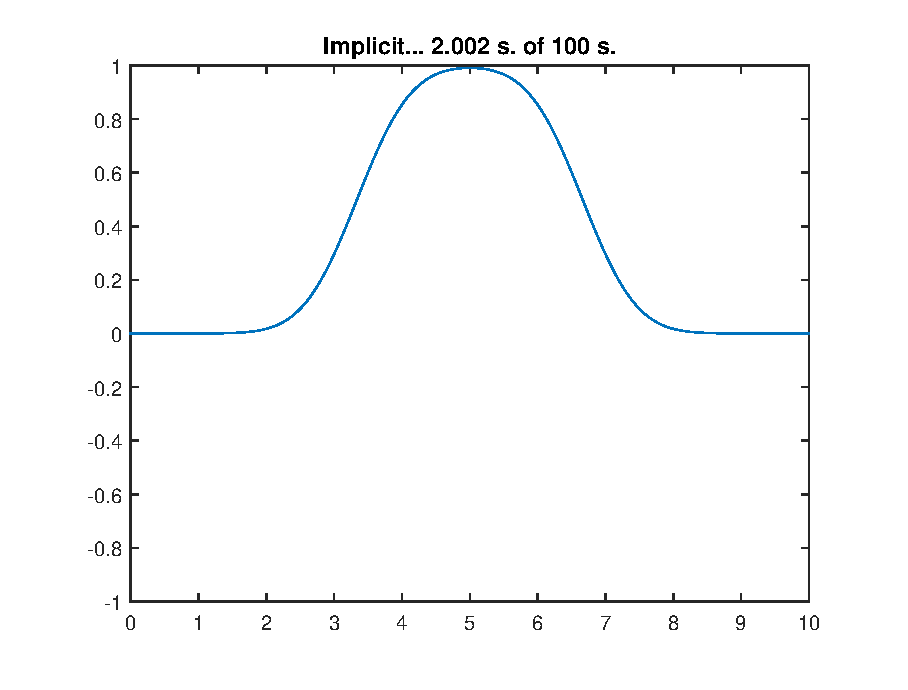
\includegraphics[width=1\textwidth]{../implicitSquare}
	\caption{Looking the implicit method solving the wave equation with initial equation 
	\ref{eq:square} after a period. While the highest point in the wave almost touch the highest point of 1 again, the square form has almost completely disappeared and it resembles more a normal function then a square.}
	\label{fig:implicitSquare}
\end{figure}

Using the fully implicit method we can see the CLF condition playing much more severe role. When using the normal and sine initial conditions (eq. \ref{eq:normal} and \ref{eq:sine}) we can clearly see severe dampening if $\Delta T < \frac{c}{\Delta x}$. Even when $\Delta T = \frac{c}{\Delta x}$ we see, if not as severe, dampening. This could of course be used to its advantage since many real life things has dampening involved, otherwise we would have a perpetual machine\footnote{Well... As long as it is without load}. This is particularly interesting in the case where we have the square wave initial condition (eq. \ref{eq:square}) since then all of a sudden instead of having oscillations around the corners we get a smoothing effect of its corners, something that very much resembles what would happen in real life. If one where to go over the CLF condition then the solutions break, no matter how small the increase is, unless of course one increases it less then the what a computer can represent in floating point. 

To conclude, the fully implicit method does have some good uses for more complex system if dampening is desired. Problem is of course that the dampening coefficient is hard to play around with since we have quite some dampening even when $\Delta T = \frac{c}{\Delta x}$, and we do not quite now how the $\Delta t$ relates to it. But for giving a general idea of a system its quite appropriate. The time step could be an issue for some systems too, making the lowest usable time step to slow to simulate within a reasonable time frame. 

\section{Fast Fourier Transform Without Time Stepping}
 \begin{figure}[H]
	\centering
	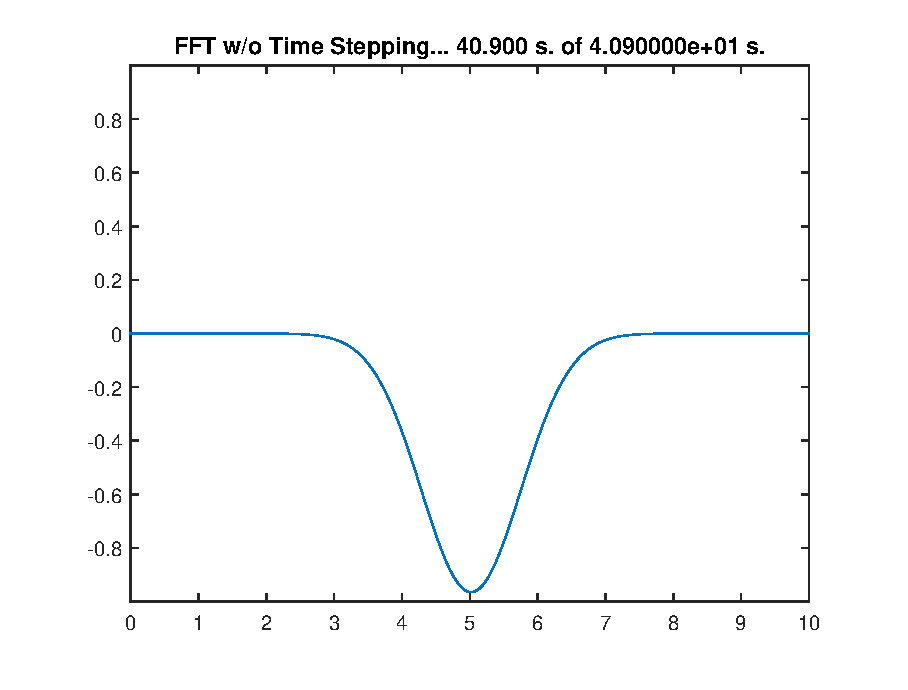
\includegraphics[width=1\textwidth]{../fftwotsNormal}
	\caption{Looking the fftwots method solving the wave equation with initial equation 
	\ref{eq:normal} after many periods. No dampening is observed and the function seem to retain is original shape}
	\label{fig:fftwotsNormal}
\end{figure}
\begin{figure}[H]
	\centering
	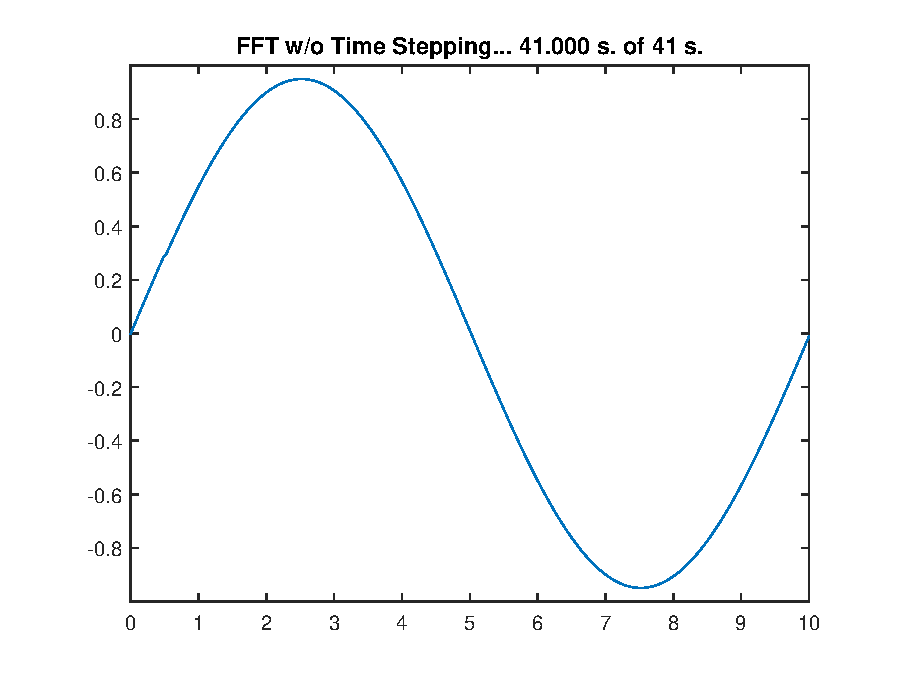
\includegraphics[width=1\textwidth]{../fftwotsSine}
	\caption{Looking the fftwots method solving the wave equation with initial equation 
	\ref{eq:sine} after many periods. No dampening is observed and the function seem to retain is original shape}
	\label{fig:fftwotsSine}
\end{figure}
\begin{figure}[H]
	\centering
	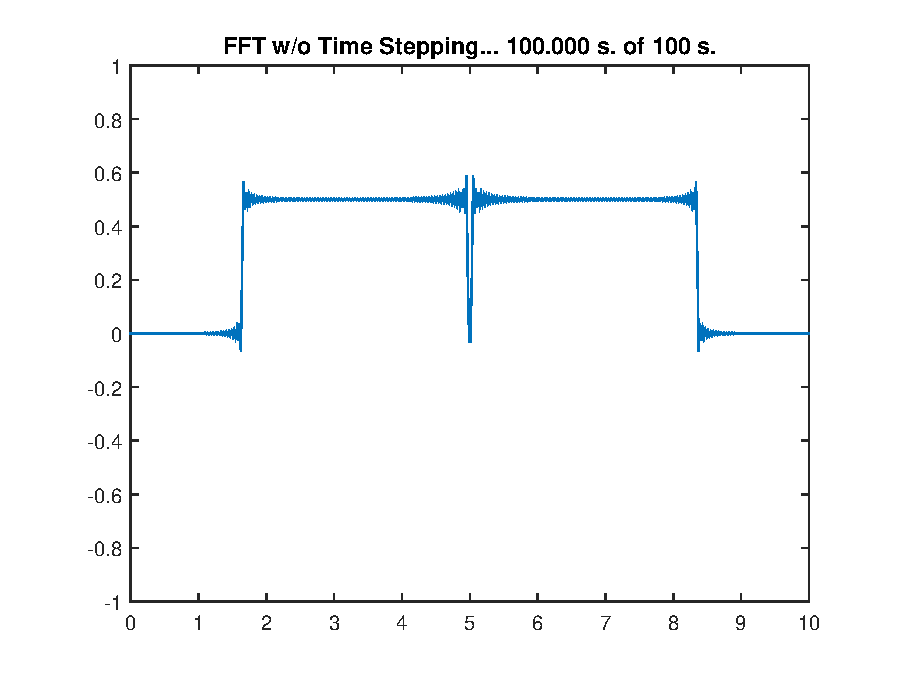
\includegraphics[width=1\textwidth]{../fftwotsSquare}
	\caption{Looking the fftwots method solving the wave equation with initial equation 
	\ref{eq:square} after after a 100 seconds. We can clearly see how the system seem to retain is original form, if the exception of oscillation around the corners.}
	\label{fig:fftwotsSquare}
\end{figure}

Looking at how to use the fourier transform without time step is a little bit less interesting then the previous methods. This since we basically solve the system analytically for different time steps instead of applying a scheme of sorts. The CLF condition basically is irrelevant in while using the method, the time step can be arbitrary small or big and the solution looks the same. One note that is a little bit interesting is how a fourier transform is made numerically. Looking at figure \ref{fig:fftwotsSquare} we can see how we have oscillations around the corners of the square, these oscillations remind the same during the whole 100 second simulation and would not change depending on the time step. This comes from the fact that the fourier transform is basically a way to transform a function in to several sine waves. So when we then solve it in the fourier space and do an inverse transform we get some oscillations since the computer cannot use an infinite amount of sine waves the represent the function. This is something to be on the guard for when using fourier transforms. 

To conclude one can say if the fourier transform method is applicable it is ideal. One has to care for sharp corners though, since this will cause ocillations since the transform is not done perfectly with a fast fourier transform. 

\section{Fast Fourier Transform With Time Stepping in K-space}
 \begin{figure}[H]
	\centering
	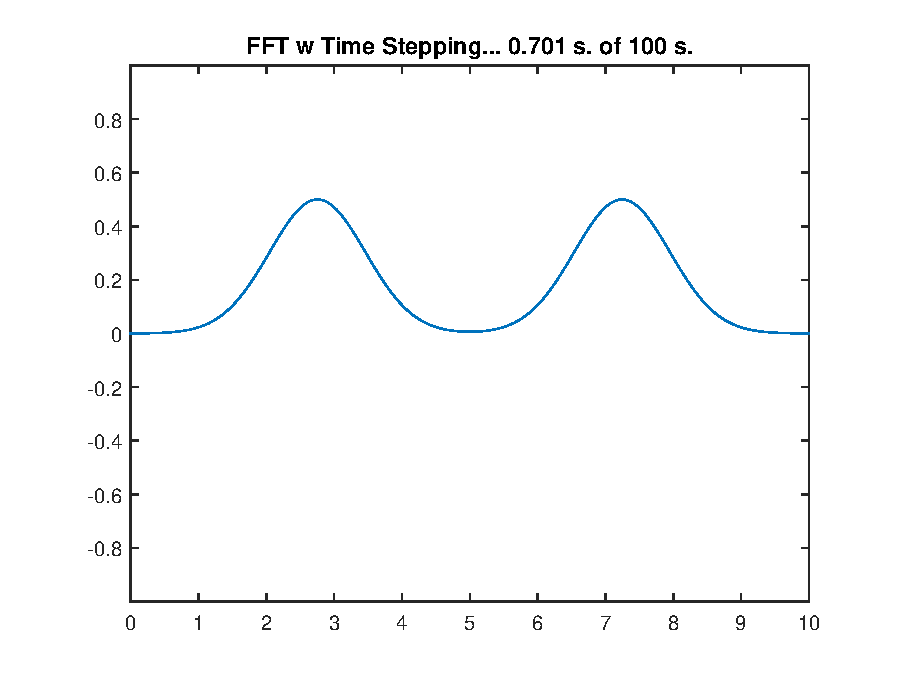
\includegraphics[width=1\textwidth]{../fftwtsNormal}
	\caption{Looking the fftwts method solving the wave equation with initial equation 
	\ref{eq:normal} after in the middle of a period. The shape is retained throughout the simulation and no artefacts are observed}
	\label{fig:fftwtsNormal}
\end{figure}
\begin{figure}[H]
	\centering
	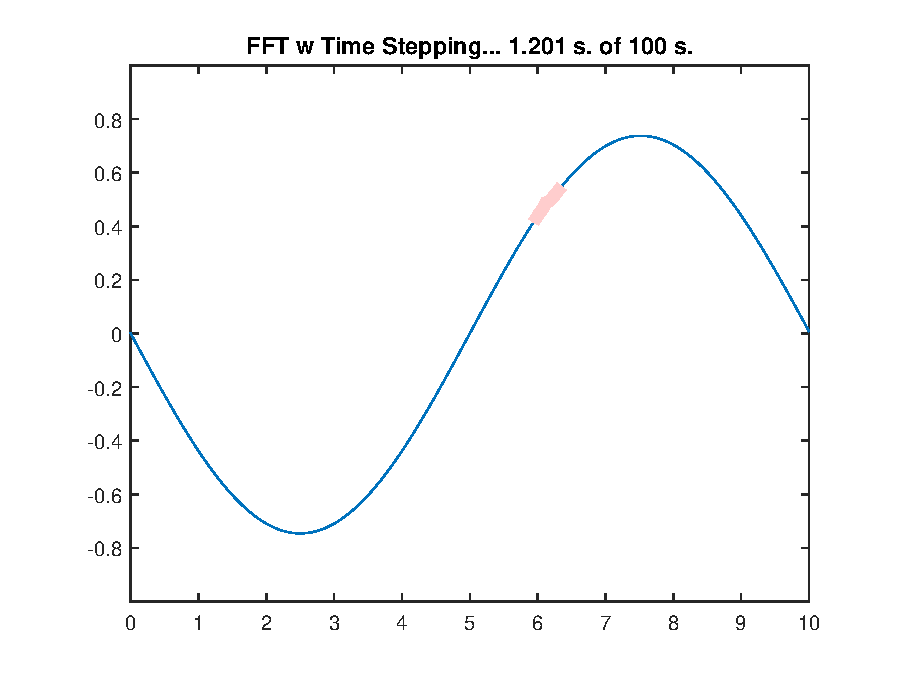
\includegraphics[width=1\textwidth]{../fftwtsSine}
	\caption{Looking the fftwts method solving the wave equation with initial equation 
	\ref{eq:sine} at its second period. We can see an artefact highlighted in red which is much more visible when the simulation is running. This occurred even if one where well below the maximum time value given by the CLF condition}
	\label{fig:fftwtsSine}
\end{figure}
\begin{figure}[H]
	\centering
	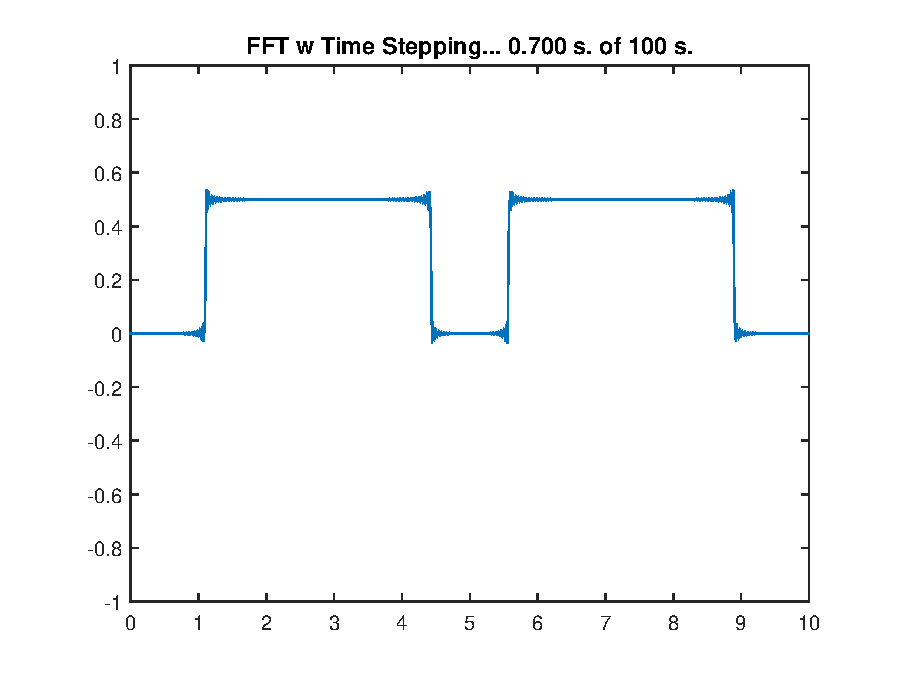
\includegraphics[width=1\textwidth]{../fftwtsSquare}
	\caption{Looking the fftwts method solving the wave equation with initial equation 
	\ref{eq:square} in its first period. The shape is retain throughout the simulation. We have some oscillation, even though it was the most accurate square wave simulation of all the methods.}
	\label{fig:fftwtsSquare}
\end{figure}

Here we needed to use a $\Delta t \leq 2 \frac{c}{\Delta x}$. Anything above this and the solutions exploded. We can see only small changes with the change with smaller time step. If one used smaller time steps the oscillations of the square wave case seem to be reduced slightly. The sine wave solution always had a small artefact that did not depend on the time step significantly. The normal wave solution looked great as long as the time step did not pass over the limit of $\frac{c}{\Delta x}$.

To conclude one can say that the square wave case was the optimally solved by this method if one does not want to see dampening as observed with the implicit method. Otherwise the FFT method without time stepping is better since you can take arbitrary time steps, which yields an unmatched efficiency, while still being accurate. 



\end{document}
